\apendice{Documentación técnica de programación}

\section{Introducción}

Este anexo describe la documentación técnica de programación.
Se incluye la instalación de IDEs, la estructura de la aplicación y el servidor, su compilación, o la configuración de diferentes servicios utilizados, con vista a que cualquier persona pueda trabajar con este proyecto o continuarlo de una forma más fácil.



\section{Estructura de directorios}

La estructura del proyecto se puede encontrar en el \href{https://github.com/fmv1001/LocalStream}{repositorio de GitHub}.\\
Dicha estructura se describe a continuación:

\begin{itemize}
\item
	\textbf{/:} Es el directorio raíz del proyecto, en el podemos encontrar el README del repositorio y el fichero de configuración de SonarQube.
\item
	\textbf{/AndroidApp/:} Contiene los ficheros de configuración de Gradle.
\item
	\textbf{/AndroidApp/app/:} módulo respectivo a la aplicación Android.
\item
	\textbf{/AndroidApp/app/src/:} En esta carpeta encontramos el código fuente de la aplicación.
\item
	\textbf{/AndroidApp/app/src/main:} la carpeta ``main'' alberga los archivos de conjunto de fuentes ``principales'': el código de la app y recursos de Android compartidos por las variantes de compilación.
\item
	\textbf{/AndroidApp/app/src/main/res/:} Contiene los recursos de aplicación, como archivos de elementos de diseño, archivos de diseño y strings de IU.
\item
	\textbf{/AndroidApp/app/src/main/java/com/example/appstream/:} Contiene las fuentes del código Java que implementa la funcionalidad de la aplicación.
\item
	\textbf{/AndroidApp/app/androidTest/:} Contiene el código necesario para las pruebas de instrumentación que se ejecutan en los dispositivos Android.
\item
	\textbf{/AndroidApp/app/test/:} Contiene el código necesario para pruebas locales.
\item
	\textbf{/docs/:} en esta carpeta se encuentra toda la documentación relativa al proyecto.
\item
	\textbf{/docs/img/:} imágenes utilizadas en la documentación relativa al proyecto.
\item
	\textbf{/docs/text/:} En la carpeta ``\textit{text}'' se encuentran los distintos documentos que forman los documentos maestros.
\item
	\textbf{/Server/:} contiene todo los archivos de código fuente necesarios para que el servidor funcione correctamente.
\end{itemize}

\section{Manual del programador}

Este manual servirá de referencia a futuros desarrolladores que trabajen en el proyecto. En el se explicaremos como preparar el entorno de desarrollo, obtener el código fuente y los requisitos necesarios para poder llevarlo a cabo.

\subsection{Requisitos}

\begin{itemize}
\item
	Python 3.
\item
	Visual Studio Code.
\item
	Android Studio.
\item
	Git.
\item
	SonarQube.
\end{itemize}

En el siguiente punto se indica como instalar y configurar correctamente cada componente.


\subsection{Entorno de desarrollo}

\subsubsection{Python 3}

Instalación de Python 3 en Windows:
\begin{enumerate}
\item
	En primer lugar debemos dirigirnos a la página oficial del Python en el apartado de \href{https://www.python.org/downloads/}{descargas}.
\item
	En segundo lugar debemos descargar el archivo de instalación pinchando en ``\textit{Download Python 3.9.7}''.
	\imagen{pythoninstall}{Página de descargas oficial de Python.}
\item
	Una vez descargado el archivo lo ejecutamos y dejando seleccionada la opción de ``\textit{Add Python to path}'', hacemos clic en ``\textit{Install Now}''
	\imagen{pythoninstall1}{Instalador para Windows de Python.}
\item
	Dejamos que termine la instalación.
	\imagen{pythoninstall2}{Instalador para Windows de Python.}
	\imagen{pythoninstall3}{Instalador para Windows de Python.}
\end{enumerate}

Instalación de Python 3 en Linux:
\begin{enumerate}
\item
	En primer lugar debemos dirigirnos a la terminal de Linux.
\item
	En segundo lugar debemos comprobar si ya lo tenemos instalado con el comando ``\textit{python3 --version}''.
\item
	Si no es así ejecutaremos el comando ``\textit{sudo apt-get install python3.6}''
\item
	Dejamos que termine la instalación y ya tenemos Python 3 instalado.
\end{enumerate}

\subsubsection{Visual Studio Code}

Instalación de Visual Studio Code:

\begin{enumerate}
\item
	En primer lugar debemos dirigirnos a la página oficial de \href{https://code.visualstudio.com/}{Visual Studio Code}.
\item
	En segundo lugar debemos descargar el archivo de instalación deseado (dependiendo de el sistema operativo que estemos usando).
\imagen{vscinstall}{Página oficial de Visual Studio Code.}
\item 
	Ahora simplemente debemos llevar a cabo los pasos del instalador.
\imagen{vscinstall3}{Instalador para Windows de Visual Studio Code.}
\imagen{vscinstall4}{Instalador para Windows de Visual Studio Code.}
\imagen{vscinstall5}{Instalador para Windows de Visual Studio Code.}
\imagen{vscinstall6}{Instalador para Windows de Visual Studio Code.}
\imagen{vscinstall7}{Instalador para Windows de Visual Studio Code.}

\item
	En linux podemos ejecutar el comando \textit{sudo apt install code} \cite{vscforrasp}
\end{enumerate}

\subsubsection{Android Studio}

Instalación de Android Studio:

\begin{enumerate}
\item
	En primer lugar debemos dirigirnos a la página oficial de Android Studio en el apartado de \href{https://developer.android.com/studio?hl=es}{descargas}.
\item
	En segundo lugar debemos descargar el archivo de instalación deseado (dependiendo de el sistema operativo que estemos usando).
\imagen{asinstall}{Página oficial de descarga de Android Studio.}
	Si pinchamos en ``\textit{Download options}'' nos dirigiremos a la página donde podemos escoger que instalador queremos exactamente para el sistema operativo usado.
\imagen{asinstall1}{Página oficial de descargas alternativas de Android Studio.}
\item 
	Ahora simplemente debemos llevar a cabo los pasos del instalador.
\imagen{asinstall2}{Instalador para Windows de Android Studio.}
\imagen{asinstall3}{Instalador para Windows de Android Studio.}
\end{enumerate}

Para este entorno de desarrollo debemos hacer una pequeña configuración inicial.
Configuración inicial de Android Studio:
\begin{enumerate}
\item
	Cuando terminamos la instalación debemos hacer esta configuración inicial que nos salta inmediatamente después.
	Simplemente debemos seguir los pasos del configuardor.
\imagen{asconfig}{Configurador para Windows de Android Studio.}
\item
	En este paso podremos elegir si queremos que se envíen nuestras estadísticas de uso a Google.
\imagen{asconfig1}{Configurador para Windows de Android Studio.}
\imagen{asconfig2}{Configurador para Windows de Android Studio.}
\imagen{asconfig3}{Configurador para Windows de Android Studio.}
\imagen{asconfig4}{Configurador para Windows de Android Studio.}
\imagen{asconfig5}{Configurador para Windows de Android Studio.}

\end{enumerate}

\subsubsection{Git}

Instalación de Git:

\begin{enumerate}
\item
	En primer lugar debemos dirigirnos a la página oficial de descargas de \href{https://git-scm.com/downloads}{Git}.
	\imagen{gitinstall}{Página oficial de git.}
\item
	En segundo lugar debemos descargar el archivo de instalación deseado (dependiendo de el sistema operativo que estemos usando).
\item 
	Ahora simplemente debemos llevar a cabo los pasos del instalador, haciendo clic en next.
\imagen{gitinstall1}{Instalador para Windows de Git.}
\imagen{gitinstall2}{Instalador para Windows de Git.}
\imagen{gitinstall3}{Instalador para Windows de Git.}
\imagen{gitinstall4}{Instalador para Windows de Git.}
\imagen{gitinstall5}{Instalador para Windows de Git.}
\imagen{gitinstall6}{Instalador para Windows de Git.}
\end{enumerate}
Una vez completado el proceso ya tenemos el entorno Git preparado, ahora cuando queramos hacer algún cambio hacia el repositorio en la nube de GitHub, simplemente debemos hacer clic derecho en la carpeta del repositorio local y hacer clic en ``\textit{Git Bash Here}''.
\imagen{gituse}{Ejemplo de cómo abrir Git Bash.}
\imagen{gituse1}{Terminal de comandos Git Bash.}

\subsubsection{SonarQube}\label{sonarQubeInstall}

Instalación de SonarQube:

\begin{enumerate}
\item
	En primer lugar debemos dirigirnos a la página oficial de descargas de \href{https://www.sonarqube.org/downloads/}{SonarQube}.
	\imagen{sqinstall}{Página oficial de descargas de SonarQube.}
\item
	En segundo lugar debemos descargar el archivo deseado.
\item 
	Cuando termine de descargarse el archivo zip, lo descomprimimos y con ese archivo ya tendremos la herramienta SonarQube.
\item 
	Si queremos iniciar SonarQube debemos ir a la carpeta \textit{/SonarQube/sonarqube-9.0.0.45539/bin/windows-x86-64/} (en el caso de Windows, hay otras para los demás sistemas operativos) del archivo descargado.
\imagen{squse}{Carpeta \textit{/SonarQube/sonarqube-9.0.0.45539/bin/windows-x86-64/}.}
\item
	Para iniciar SonarQube debemos ejecutar el archivo ``\textit{StartSonar.bat}'' y esperar a su ejecución, nos dirigimos a un navegador y vamos a la dirección ``\textit{http://localhost:9000/}'' e iniciamos sesión.
\imagen{squse1}{Pantalla incial de SonarQube.}
\imagen{squse2}{Pantalla principal de SonarQube.}\label{princiQube}
\item
	Para parar SonarQube debemos ejecutar ``\textit{Ctrl + c}'' en la terminal de ejecución de SonarQube.
\end{enumerate}

Para escanear documentos SonarQube provee la herramienta SonarScanner.\\
Instalación de SonarScanner:

\begin{enumerate}
\item
	En primer lugar debemos dirigirnos a la página oficial de descargas de \href{https://docs.sonarqube.org/latest/analysis/scan/sonarscanner/}{SonarQube} para SonarScanner.
	\imagen{ssinstall}{Página oficial de SonarQube de descarga de SonarScanner.}
\item
	En segundo lugar debemos descargar el archivo deseado.
\item 
	Cuando termine de descargarse el archivo zip, lo descomprimimos y con ese archivo ya tendremos la herramienta SonarScanner de SonarQube.
\end{enumerate}

Antes de poder usar SonarScanner debemos hacer un pequeña configuración.\\

Configuración de SonarScanner:

\begin{enumerate}
\item
	En primer lugar debemos ir a la carpeta \textit{/sonar-scanner-4.6.2.2472-windows/conf} del archivo descargado.
\imagen{ssconf}{Carpeta \textit{/sonar-scanner-4.6.2.2472-windows/conf}.}
\item
	En segundo lugar debemos modificar el archivo \textit{sonar-scanner.properties} o crear un archivo con la extensión ``\textit{.properties}''.
\item 
	El archivo de configuración debe contener lo siguiente:
	\begin{itemize}
	\item
		Una clave de proyecto o \textit{sonar.projectKey}.
	\item
		Un nombre para el proyecto o \textit{sonar.projectName}.
	\item
		Un patch para la fuente de archivos de código o \textit{sonar.sources}.
	\imagen{ssconf1}{Ejemplo de archivo de configuración de SonarScanner.}
	\end{itemize}
\end{enumerate}



\section{Compilación, instalación y ejecución del proyecto}

Antes de proceder a la compilación, instalación y ejecución del proyecto debemos descargar el \href{https://github.com/fmv1001/LocalStream}{repositorio de GitHub}.
Para ello copiamos la dirección del repositorio (\textit{https://github.com/fmv1001/LocalStream}) y en la herramienta Git Bash for Windows ejecutamos el comando ``\textit{git clone https://github.com/fmv1001/LocalStream}'', que clonara el repositorio en una carpeta local de nuestro dispositivo.
\imagen{descargaRep}{Descarga del repositorio a través de comandos Git.}

\subsection{Importar el proyecto en Android Studio}

Cuando ya tenemos el código del proyecto en el dispositivo, ya podemos comenzar a prepara el entorno Android. En este punto debemos seguir una serie de pasos:
\begin{enumerate}
\item
	Abriremos Android Studio.
\item
	Nos desplazaremos hasta la esquina superior izquierda y pinchamos en \textit{File > New > Import Project...}
	\imagen{asimport}{Importar proyecto en Android Studio.}
\item
	Una vez lleguemos a este momento, debemos navegar hasta la carpeta en la que hemos clonado el proyecto y seleccionar la carpeta \textit{AndroidApp} y hacer clic en \textit{Seleccionar carpeta}.
\imagen{asimport1}{Importar proyecto en Android studio}
\item
	En este punto sólo debemos esperar a que Gradle se encargue de configuarar y preparar el proyecto para el entorno Android Studio.
\imagen{asimport2}{Proyecto importado en Android studio}
\end{enumerate}

Si queremos ver más detalladamente como realizar este paso dirigirse a \cite{importAS}.

\subsubsection{Importar el proyecto en Visual Studio Code}\label{importtovsc}

Una vez instalada la herramienta Visual Studio Code:

\begin{enumerate}
\item
	Abriremos Visual Studio Code.
\item
	Nos desplazaremos hasta la esquina superior izquierda y pinchamos en \textit{File > Open Folder...}
	\imagen{vscimport}{Importar proyecto en Visual Studio Code.}
\item
	Una vez lleguemos a este momento, debemos navegar hasta la carpeta en la que hemos clonado el proyecto y seleccionar la carpeta \textit{Server} y hacer clic en \textit{OK}.
\imagen{vscimport1}{Importar proyecto en Visual Studio Code}
\item
	En este punto sólo debemos esperar a que Visual Studio Code preparar el proyecto.
\imagen{vscimport2}{Proyecto importado en Visual Studio Code}
\end{enumerate}

\subsection{Añadir funcionalidad al sistema}

Una vez importados los dos proyectos en sus respectivos entornos de desarrollo integrado, podemos realizar las modificaciones requeridas.\\
Si queremos añadir alguna funcionalidad manteniendo el modelo Cliente-Servidor, debemos seguir como mínimo los siguientes pasos:

\begin{enumerate}
\item
	Crear una nueva rama en desde la rama principal (\textit{main}) del proyecto desde Git Bash:\\
	\textit{git checkout -b export-data main}
\item
	1.
\end{enumerate}

\subsection{Actualizar dependencias del proyecto}

Para que nuestra aplicación se mantenga actualizada debemos actualizar las versiones o dependencias del proyecto, en este caso las de la aplicación y el servidor.\\

En primera instancia vamos a proceder a la explicación de cómo hacer esta actualización sobre la aplicación:

\begin{enumerate}
\item
	En primer lugar nos vamos a dirigir al archivo \textit{build.gradle}, ya que Gradle es el sistema de construcción de software de Android y una de las funciones que realiza es la gestión de dependencias. Este archivo se encuentra en la carpeta de la aplicación, \textit{/AndroidApp/}, y contiene las dependencias de la aplicación.
\item
	Nos situaremos en esa carpeta desde la herramienta Android Studio y abriremos el archivo. 
\imagen{asdependencies}{Dependencias de la aplicación}
\item
	Podemos observar que disponemos de distintos tipos de dependencias:
	\begin{itemize}
		\item
			implementation:
			Gradle agrega la dependencia a la ruta de clase de la compilación y la empaqueta en el resultado de la compilación
		\item
			testImplementation: 
			Gradle empaqueta esta dependencia para los test de la aplicación.
		\item
			androidTestImplementation: 
			Gradle la empaqueta para los test de instrumentación de la aplicación.			
	\end{itemize}
	Existes otros tipos de dependencias, que podemos encontrar en \cite{androiddepend}.
\item
	A lo hora de actualizar cada una de ellas debemos actualizar el número de versión de la dependencia por el número de la versión deseado.
	\imagen{asdependencies1}{Dependencia en Android}
\item
	Después debemos ir a \textit{File > Sync Project with Gradle Files} y Gradle sincronizará el proyecto con las nuevas dependencias.
\imagen{asdependencies2}{Sincronización del proyecto con las nuevas dependencias.}
\end{enumerate}

Para actualizar las dependencias en el servidor, debemos hacerlo sobre Python:

\begin{itemize}
\item
	En Linux debemos ejecutar el siguiente comando:\\
	\textit{sudo pip install -U nombrePaquete}
\item
	En Windows en la instalación de python se agrega al path el comando \textit{pip} y debemos ejecutar:\\
	\textit{pip install nombre-paquete --upgrade}
\item
	Para actualizar a una versión específica debemos ejecutar en el terminal (para Windows o Linux):\\
	\textit{pip install nombre-paquete == 1.0.0}
\end{itemize}

\subsection{Compilación del código del proyecto}

\subsubsection{Aplicación}

Para compilar la aplicación debemos hacer uso de Gradle. Para ello nos dirigimos a la parte superior de Android Studio y seleccionamos \textit{Build -> Make Project}.
\imagen{ascomp}{Compilación de la aplicación desde Android Studio.}

\subsubsection{Servidor}

La compilación del servidor se realizará durante la ejecución del mismo.

\subsection{SonarQube}

SonarQube es una plataforma de código abierto desarrollada en Java que nos permite realizar análisis de código con diferentes herramientas de forma automatizada.
Vamos a proceder a la explicación de como lo hemos integrado al proyecto, y cómo usarlo.\\
\begin{enumerate}
\item
	Una vez instalado e inciado SonarQube como se explica en \ref{sonarQubeInstall} debemos dirigirnos a la carpeta del repositorio del proyecto y abrir una terminal. 
	Podemos hacerlo desde la ruta escribiendo \textit{cmd}\ref{abrircmd} o desde el terminal navegar hasta la ruta.
\imagen{ssuse1}{Cómo abrir un terminal desde una carpeta en Windows.}\label{abrircmd}
\item 
	Una vez llegado este momento, debemos ejecutar uno de los siguientes comandos:
	\begin{itemize}
	\item
		Si no tenemos un archivo de configuración:\\
		\textit{sonar-scanner -Dsonar.projectKey=Key1 -Dsonar.projectName=LocalStream -Dsonar.sources=Server/ -Dsonar.login=} ``\textit{admin}'' \textit{-Dsonar.password=}``\textit{****}''
	\item
	Si tenemos un archivo de configuración:\\
		\textit{sonar-scanner -Dproject.settings=sonar-project.properties -Dsonar.login=} ``\textit{admin}'' \textit{-Dsonar.password=}``\textit{****}''
	\end{itemize}
\item
	Después, esperamos a que termine la ejecución del comando. Cuando haya terminado nos dirigimos a la página principal de SonarQube \ref{princiQube}. 
\item
	Una vez allí nos dirigimos a la pestaña \textit{Issues} en el borde superior. Allí nos muestra todos los bugs, las vulnerabilidades y ``code smell'' que hay en el código y debería ser corregido. 
\imagen{ssuse2}{Pestaña \textit{Issues} de SonarQube}
\end{enumerate}

\subsection{Ejecución del sistema}

\subsubsection{Ejecución de la aplicación}

La ejecución de la aplicación puede hacerse de diferentes maneras:\\
\textbf{En el emulador android de Android Studio}\\
Un emulador simula el funcionamiento de un dispositivo, en este caso el emulador que usaremos es \textit{Android Simulator} que genera instancias de \textit{Android Virtual Device o AVD}. 
Para poder usar el emulador de android debemos disponer de un sistema operativo de 64 bits (para saber más ir \cite{andsim}).
Para ejecutar nuestra aplicación en este emulador debemos seguir estos pasos:
\begin{enumerate}
\item \label{avdemulator}
	Primero situese en el administrador de AVD de android.
\imagen{asemul}{Administrador de Android Virtual Devices.}
\item
	Después ejecute el emulador en el icono triangular verde.
\imagen{asemul1}{Android Virtual Device.}
\item
	Si no tenemos un AVD debemos crearlo pulsando en ``\textit{Create New Virtual Device}'' con las características que deseemos. Después de finalizar volvemos al paso \ref{avdemulator}.
\end{enumerate}

\textbf{En un dispositivo Android}\\

Para ejecutar nuestra aplicación en este emulador antes debemos instalar los drivers necesarios. Lo haremos desde el borde superior \textit{Tool -> SDK Manager}, y debemos tener instala la opción \textit{Google USB Driver}.
\imagen{asusbdriver}{Android SDK options.}
Después, para conectar un disposito Android al PC que estemos usando, debemos activar la depuración USB del dispositivo \cite{andusbdebug}.
Luego seguiremos estos pasos:
\begin{enumerate}
\item
	Primero sitúese en el administrador de AVD de android.
\item
	Después ejecute el emulador en el icono triangular verde cuando este muestre el nombre de su dispositivo Android.
\imagen{asemul2}{Administrador de Android Virtual Devices.}
\begin{figure}[h!]
	\centering
	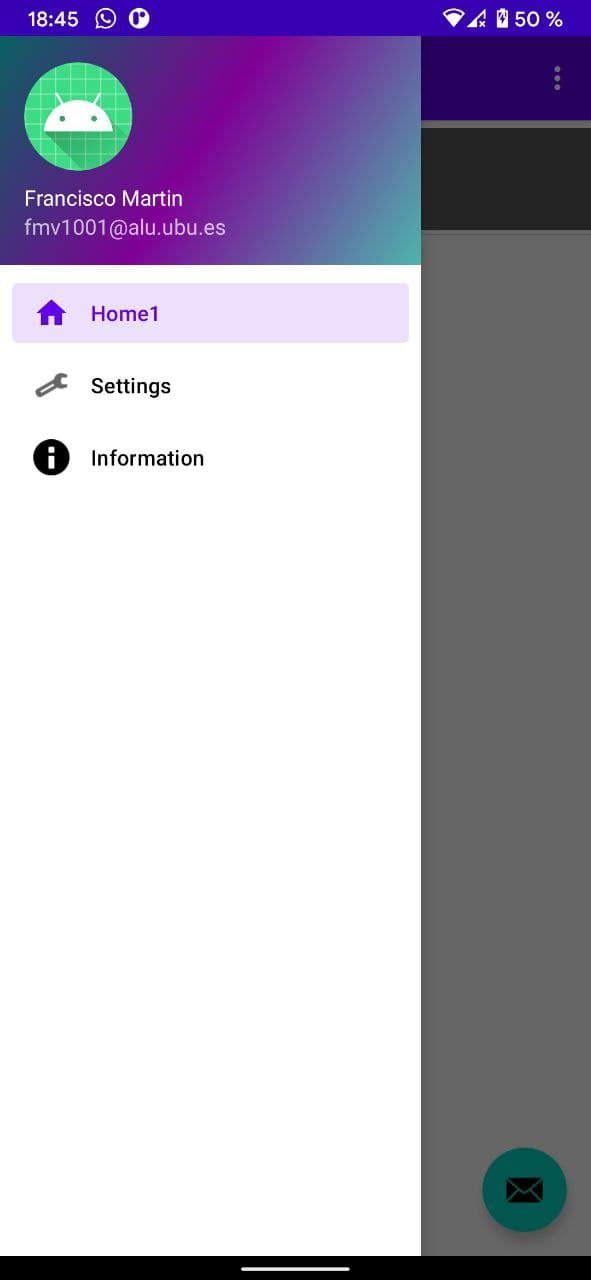
\includegraphics[width=0.35\linewidth]{img/appdevice}
	\caption{Aplicación ejecutada en dispositovo Android.}
	\label{fig:androapp}
\end{figure}
\end{enumerate}

\textbf{Generar APK de la aplicación}\\
Para generar el APK debemos realizar los siguientes pasos:
\begin{enumerate}
\item
	Primero debemos dirigirnos a la barra superior y ir al menú \textit{Build -> Generate Signed Bundle/APK}.
\imagen{asapk}{Menú Build de Android Studio para generar APK.}
\item
	Después, seleccionamos la opción APK y hacemos clic en \textit{Next}.
\imagen{asapk1}{Menú Build de Android Studio para generar APK.}
\item
	Después, seleccionamos la firma a usar o creamos una nueva desde \textit{Create new...} y hacemos clic en \textit{Next}.
\imagen{asapk3}{Menú \textit{Generate Signed Bundle/APK}.}
\imagen{asapk2}{Menú \textit{New key Store}.}
\item
	Después, seleccionamos \textit{release} y la opción \textit{V2 (Full APK Signature)} para que se cree el APK ya firmado, y hacemos clic en \textit{Finish}. Ahora sólo debemos esperar a que Gradle genere el archivo APK.
\imagen{asapk4}{Menú \textit{Generate Signed Bundle/APK}.}
\item
	Una vez generado lo podremos encontrar en la carpeta \textit{/AndroidApp/app/release/}
\end{enumerate}

Después de generar el archivo lo pasamos al teléfono y lo ejecutamos, misma salida que \ref{fig:androapp}.

\subsubsection{Ejecución del servidor}

Para la ejecución del servidor deberemos haber instalado previamente Visual Studio Code y Python 3 en el dispositivo que queramos desplegarlo.\\
Una vez instalados los componentes, abrimos Visual Studio Code, importamos el proyecto (tal como se explica en manual \ref{importtovsc}).
Después abrimos el archivo MainServer.py y en la esquina superior derecha ejecutamos pinchando el el icono \textit{play/run}. 
Seguidos estos pasos el servidor ya se encuentra en ejecución.
\imagen{runvsc}{Ejecución del servidor desde Visual Studio Code.}

También podemos ejecutar el servidor desde comandos situándonos en la carpeta \textit{/Server/} y desde el terminal ejecutamos el comando:\\
\textit{python3 MainServer.py}



\section{Pruebas del sistema}













